%----------------------------------------------------------------------------------------
%	SLIDE 4.
%----------------------------------------------------------------------------------------
\begin{frame}
\frametitle{Results - Degree distribution}

\begin{figure}
	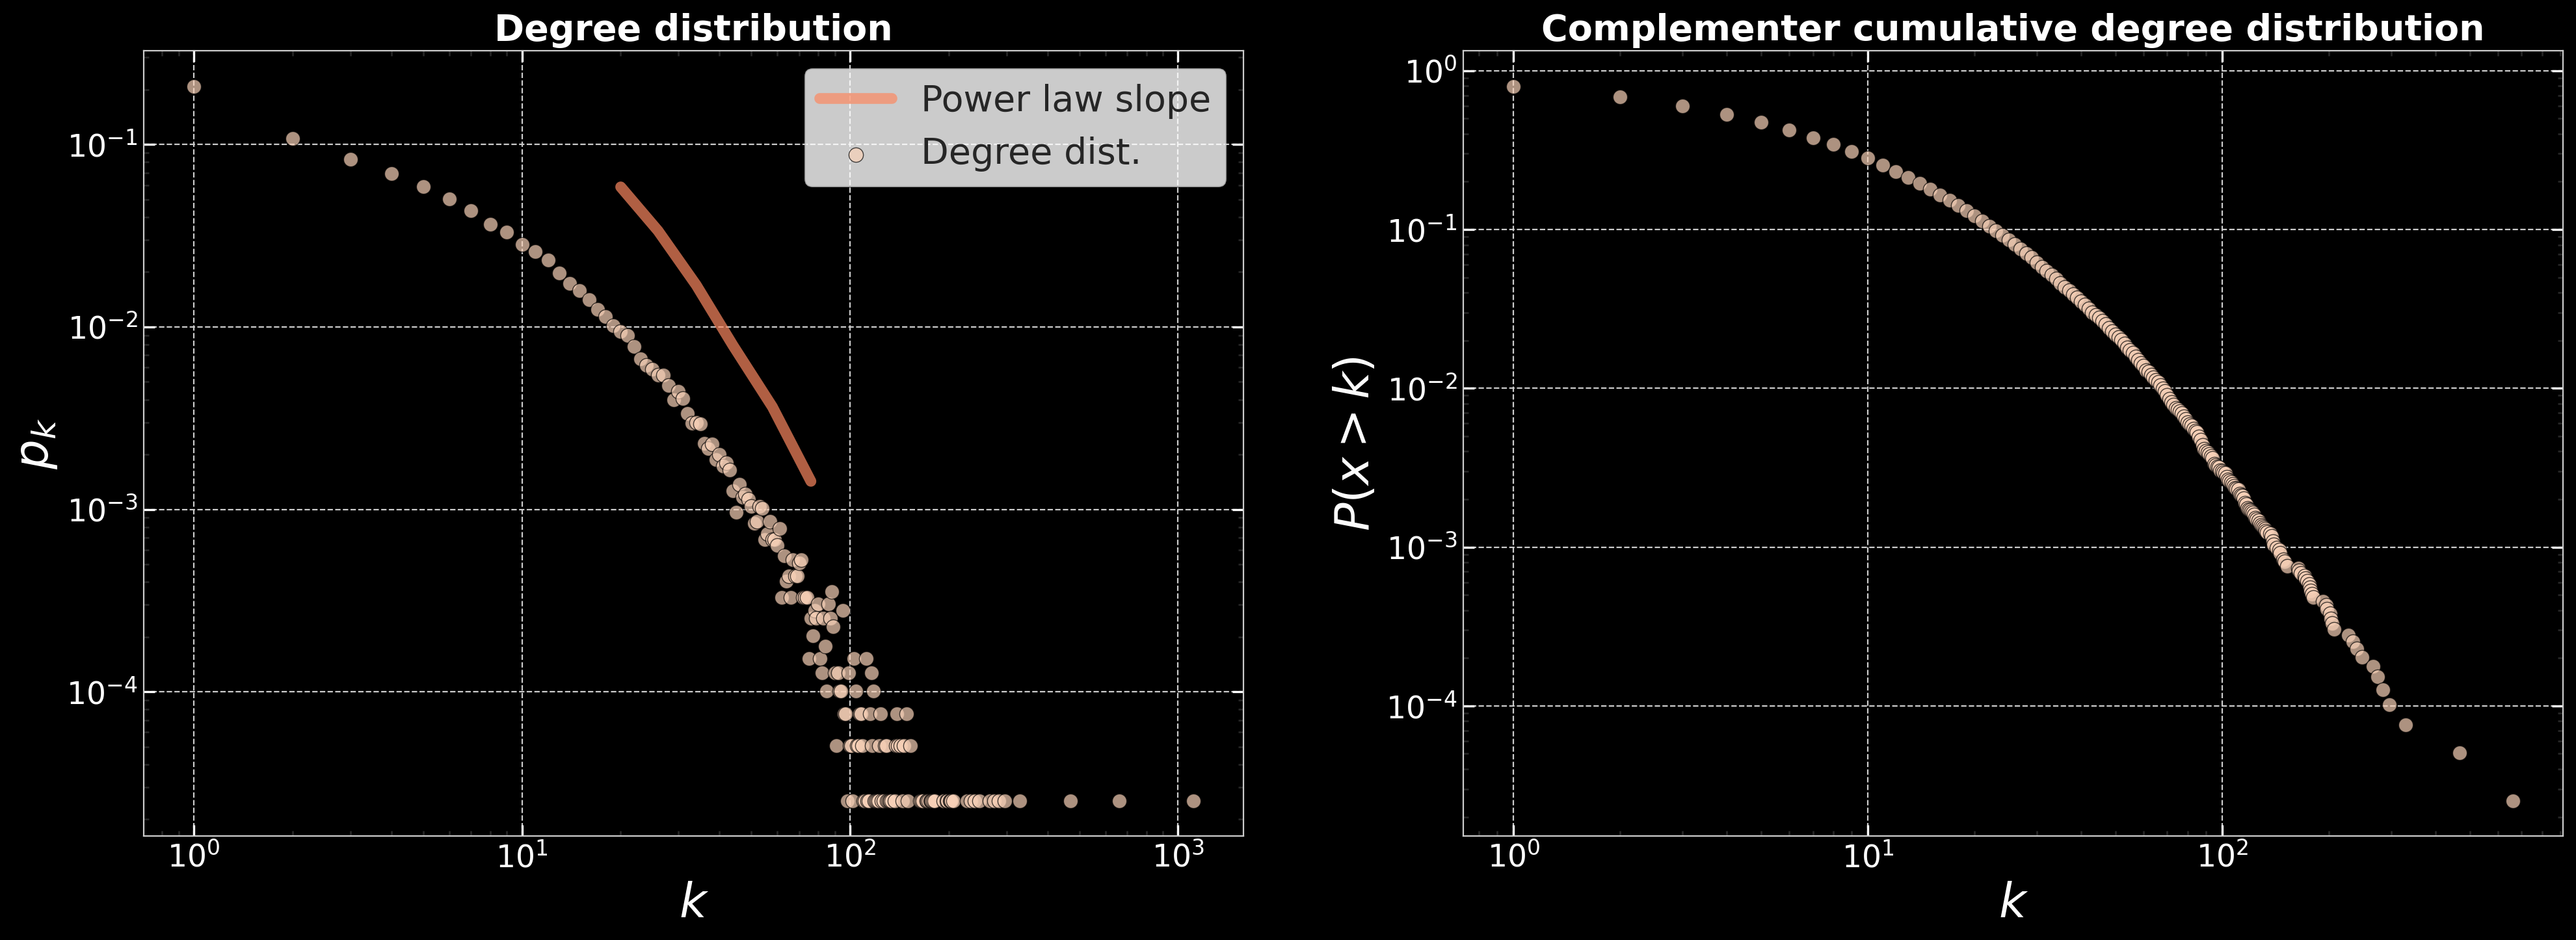
\includegraphics[width=\textwidth]{./images/degdist_small.png}
	\captionof{figure}{Degree distribution (left) and complementer cumulative degree distribution (right) of the selected nodes around Missouri. The degree distribution follows the power law, $P \left( k \right) \sim k^{-\gamma}$, which indicates the selected sub-graph is could be a scale-free network between $20 < k < 100$. In this interval the exponent $\gamma = 2.604 \pm 0.023$. The clustering coefficient $C = 0.172$ \footnote{For a much larger dataset in the original article these values were $\gamma = 2.60 \pm 0.01$ and $C = 0.14$.}.}
\end{figure}

\end{frame}